\documentclass[12pt]{article}
\usepackage{preamble}

\author{Francisco Pessoa (1°EM A, N°6)}
\title{Trabalho \textbf{Minha geografia}}
\date{\today}

\begin{document}

\maketitle

\section{Meu quarto}
\subsection{Descrição da paisagem}
\url{http://0x0.st/Xso_.mp3}
\subsection{Análise do espaço}
Podemos deduzir, a partir do silêncio quase absoluto da gravação no meu quarto, muito sobre a minha condição social. Eu tenho um tempo e um espaço que não atrapalham para, por exemplo, estudar — tenho completa liberdade, algo que certamente me ajudará na minha trajetória acadêmica. Em uma cidade grande como São Paulo, é difícil encontrar tal calma e falta de barulho: é um privilégio imenso poder usufruir disso.

\section{Ponto de ônibus do ICB}
\subsection{Descrição da paisagem}
\begin{figure}[H]
    \centering
    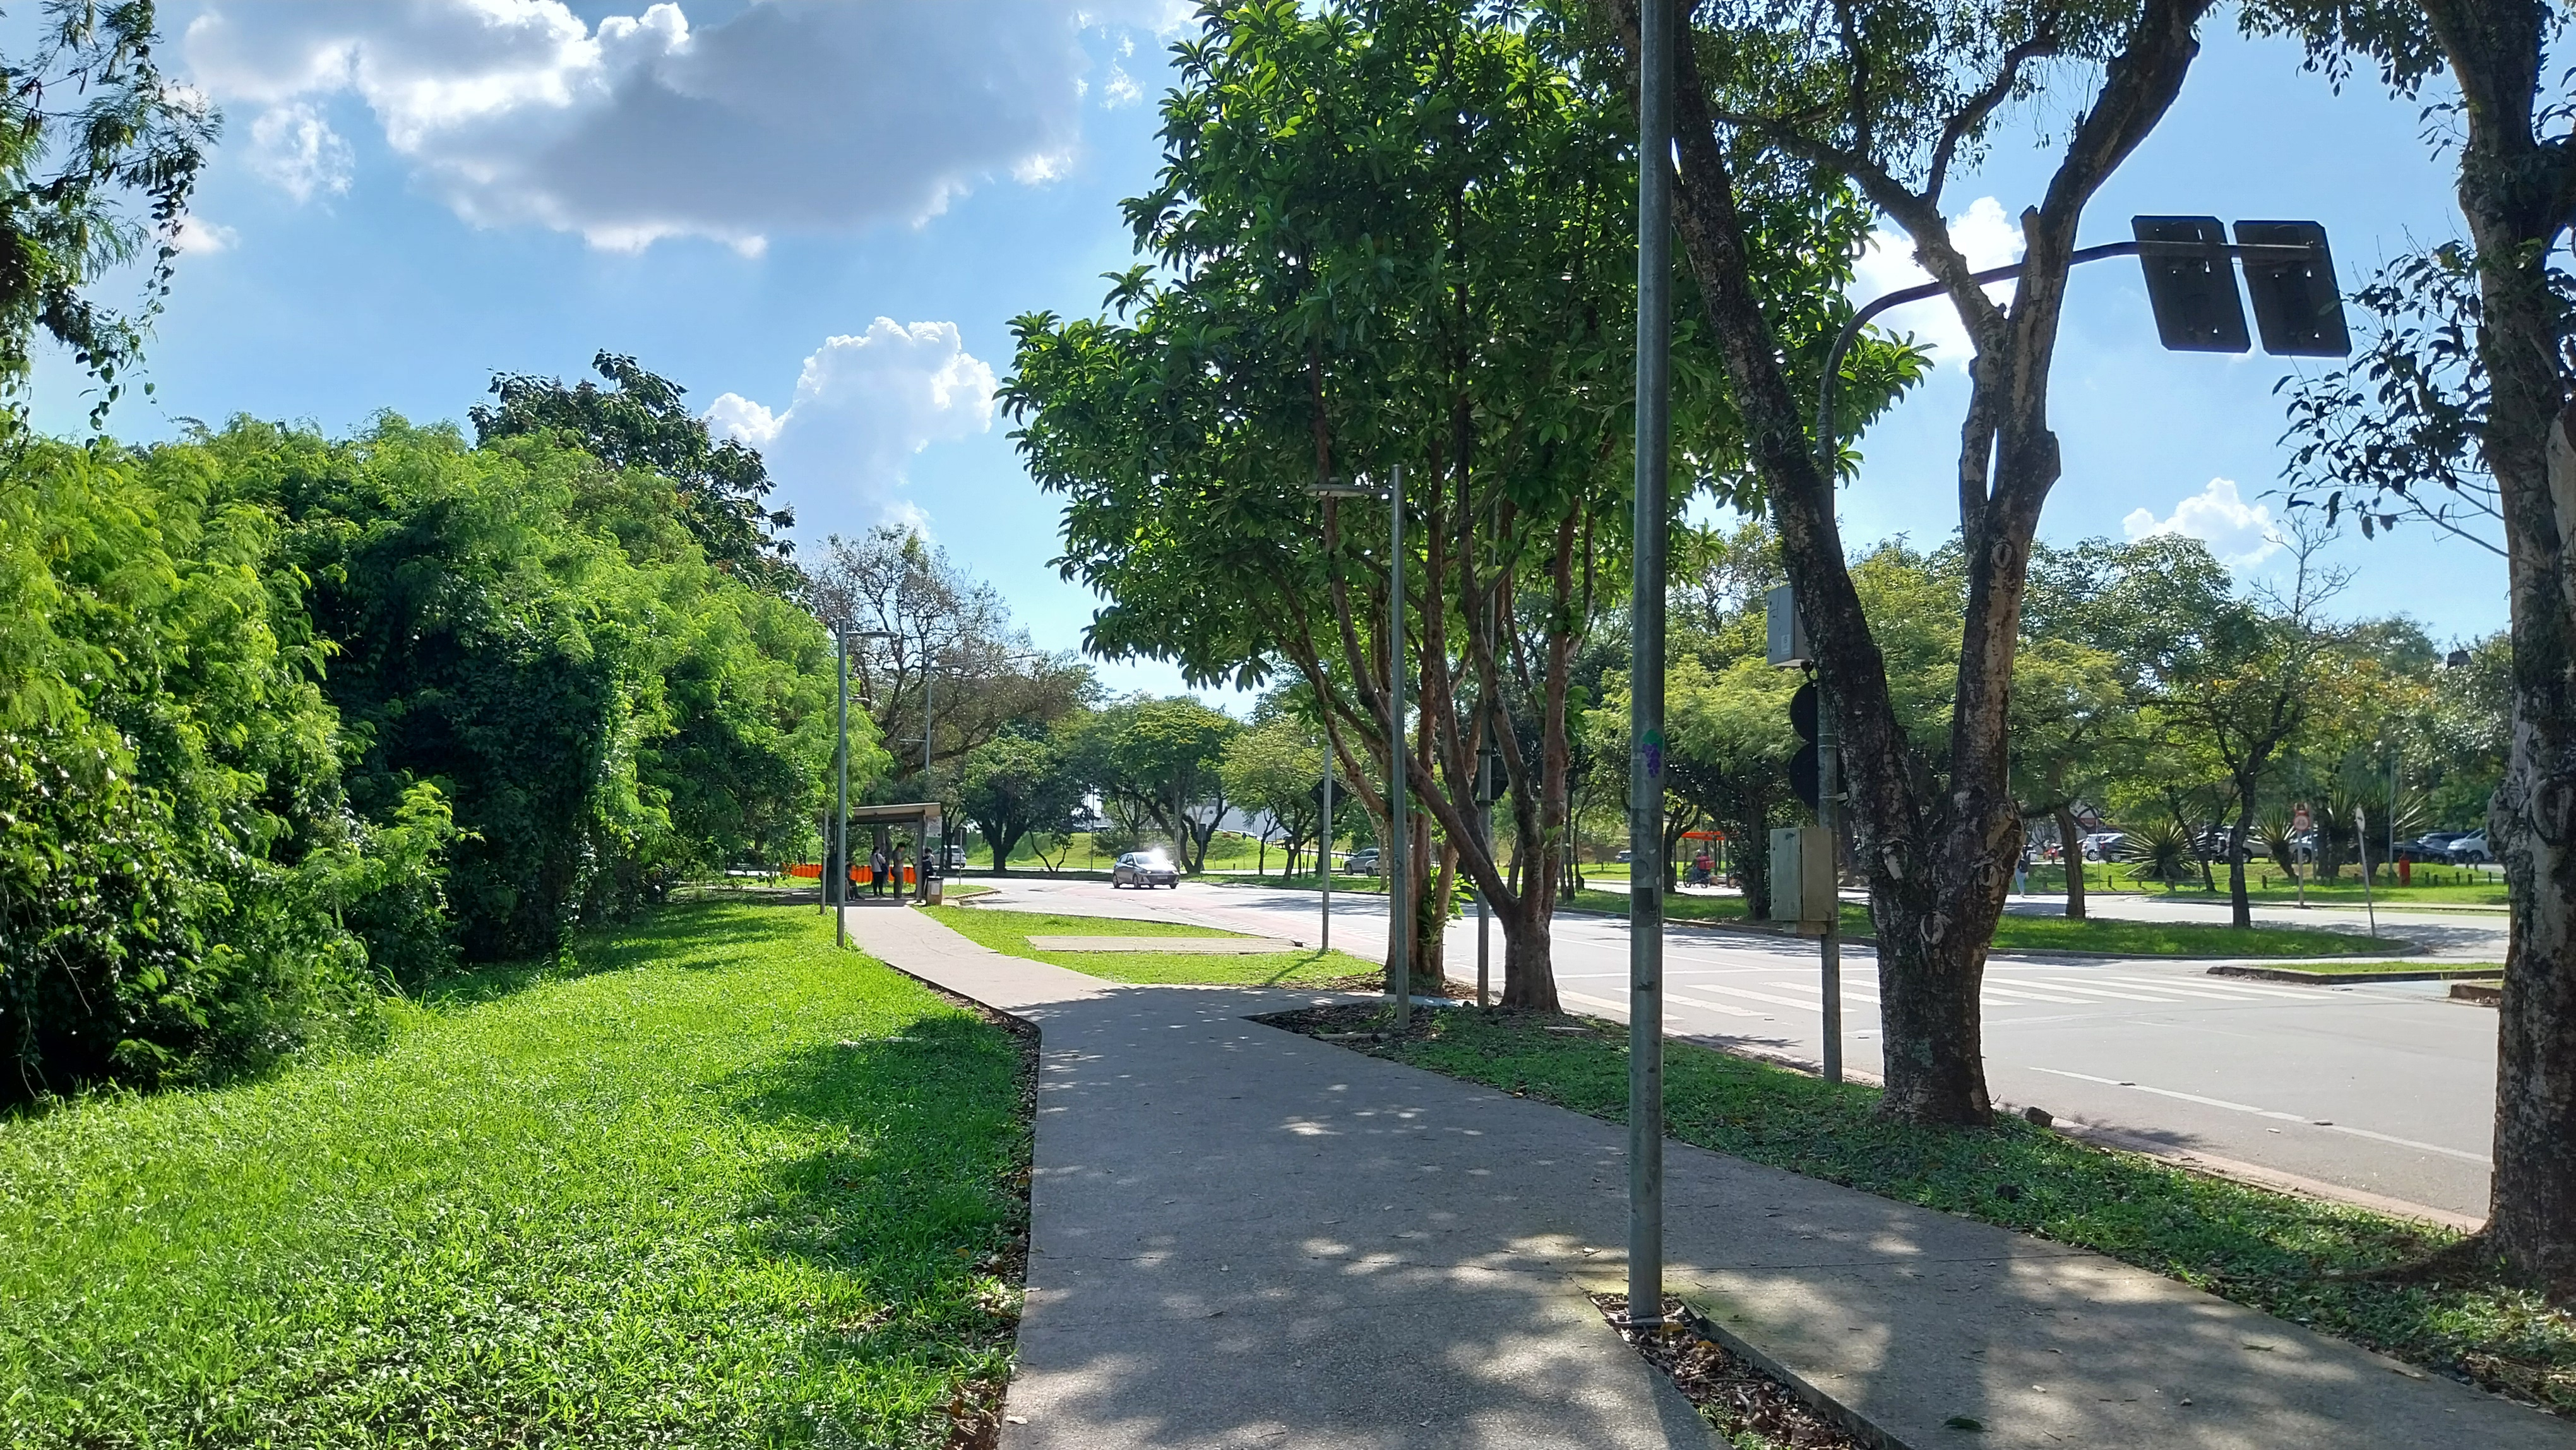
\includegraphics[width = \textwidth]{./img/Ponto.jpg}
\end{figure}
\subsection{Análise do espaço}
O ponto de ônibus do ICB, na USP, foi onde peguei ônibus sozinho pela primeira vez, em 2022. Isso me deu muito mais independência para andar pela cidade, facilitando o encontro com amigos, e quebrou a clássica preocupação de pais de classe média em relação ao perigo de andar sozinho na cidade. Foi algo muito transformador nesse sentido, me revelando muito sobre a cidade, suas coisas boas e ruins, e o dia a dia de uma vida adulta.

Existe algo a ser dito, nesse sentido, sobre o fato da primeira vez que eu andei de ônibus ter sido com 12/13 anos: é muito mais tarde do que a maioria das pessoas, o que também revela muito sobre a minha condição social: significa que eu sempre tive um carro, ou uma perua escolar, ou um táxi, por exemplo, para me levar onde precisasse ir. Eu nunca tivera, até aquele momento, a necessidade de andar de transporte público; e mesmo minhas primeiras vezes foram por motivos fúteis dentro do que seria um ``ambiente controlado'', na Cidade Universitária. Motivos que realmente fizeram com que fosse necessário o meu uso de ônibus só apareceram muito mais tarde: por volta do fim de 2023, quando precisei voltar da escola.

Essa preocupação de pais de classe média com os filhos andado pela cidade fornece-nos uma ótima mobilização do conceito de lugar. Para eles, a cidade preenche um lugar de dificultador das relações sociais, algo que deve ser evitado. Essas preocupações com segurança pública são inteiramente válidas, mas algumas vezes apresentam-se mais importantes do que o próprio crescimento e independência dos filhos, diferentemente de pais que não tenham condições de pagar (ou tempo de dar) transporte, onde os filhos são obrigados desde mais cedo a romper com essa abstração da cidade e colocá-la no lugar de um meio indiferente pelo qual se dá a locomoção, comércio, as relações sociais, entre outros.

Por fim, toda essa história enfatiza a minha conexão com a USP. Moro a um quarteirão de distância da entrada de pedestres da Vila Indiana, um bairro quase inteiramente formado por repúblicas estudantis. Foi onde eu mais saí durante a pandemia, quando andava por suas ruas desertas, e é um lugar que me fez viver muitas experiências diferentes. 

\section{Movimento, a minha escola de música}
\subsection{Descrição da paisagem}
\url{http://0x0.st/Xso2.mp3}
\subsection{Análise do espaço}
Podemos ver aqui um espaço cultural e um grupo de adolescentes desafinados. 
Brincadeiras a parte, é um espaço que mostra muito bem o quão privilegiado eu sou, ao conseguir pagar para 4h de aulas de música por semana. Além disso, mostra questões geopolíticas, sobre a influência cultural num mundo globalizado tal que uma banda brasileira toca praticamente só músicas em inglês, com instrumentos que não são típicos de nossa região, demonstrando um certo ``desprezo'' pela música e cultura brasileira.


\section{Arco, minha escola do sexto ao sétimo ano}
\subsection{Descrição da paisagem}
\subsubsection{Exterior}
\begin{figure}[H]
    \centering
    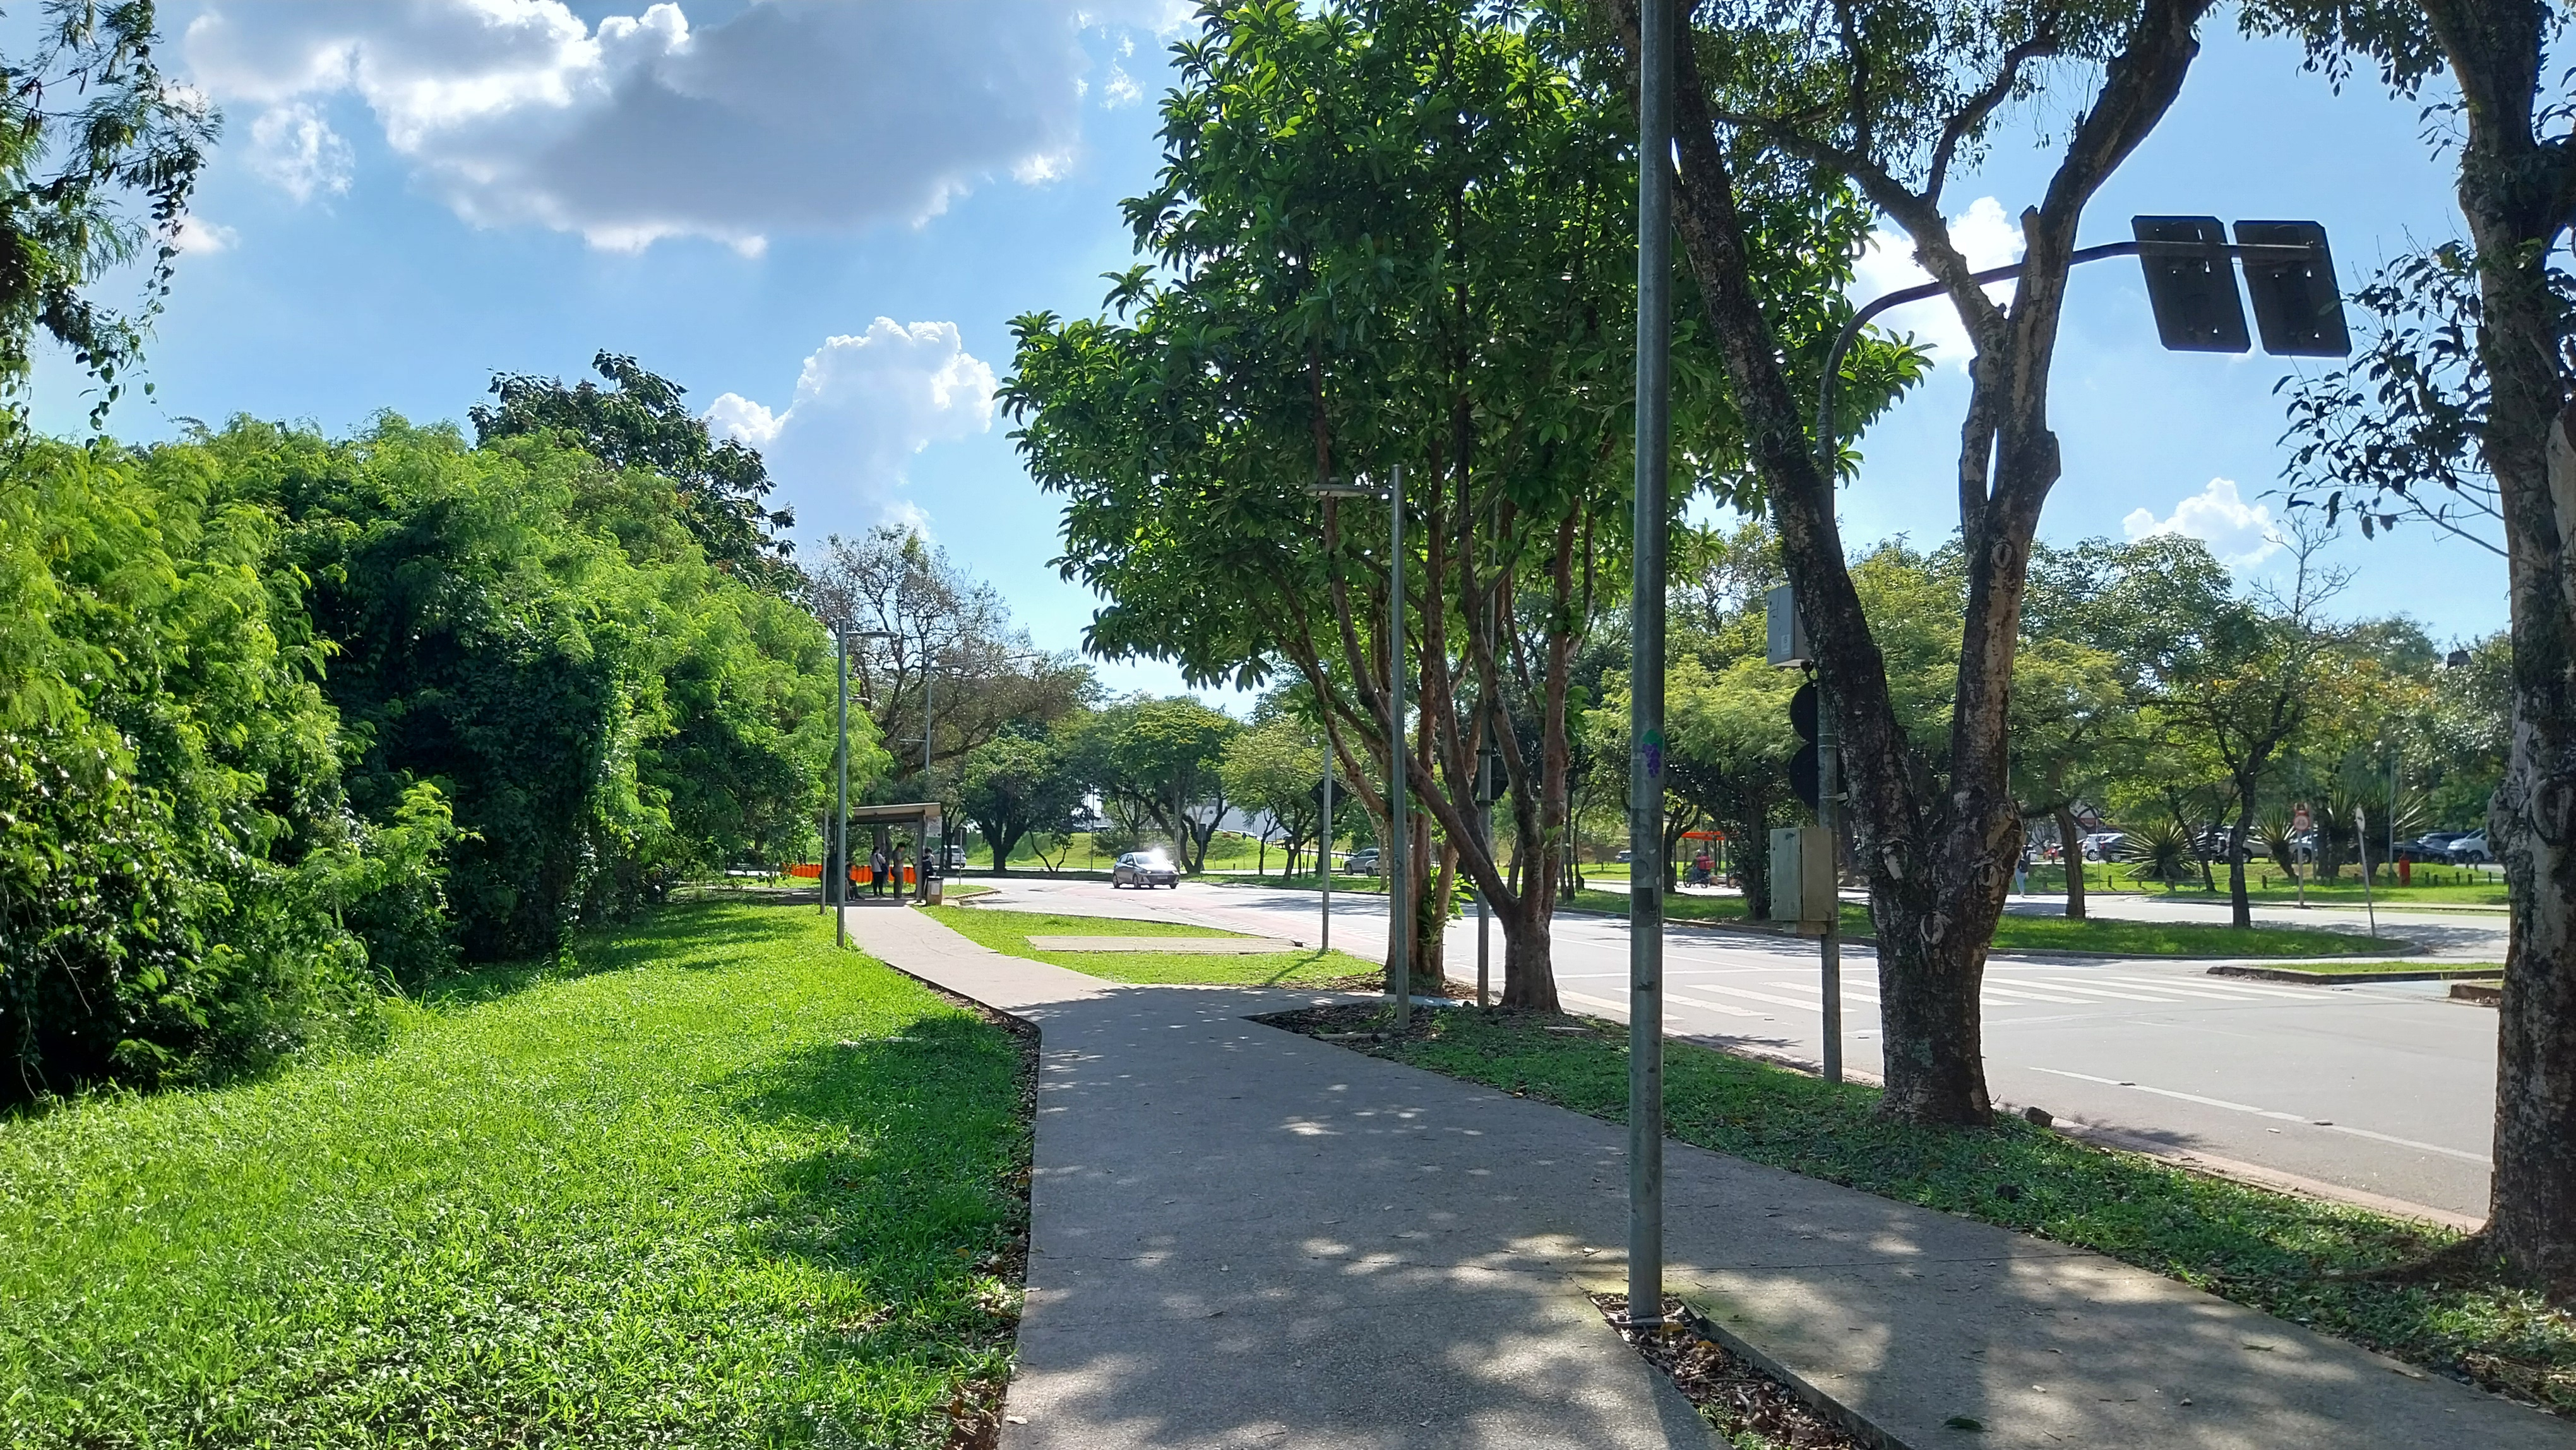
\includegraphics[width = \textwidth]{./img/Ponto.jpg}
\end{figure}
\subsubsection{Interior}
Por dentro da Arco há uma pequena arena semicircular com plateia ao ar livre, que dá acesso a um amplo salão interno. Neste, há portas para algumas salas, como o ateliê, laboratório, oficina e auditório, uma grande cozinha com lavanderia ao fundo e uma escada que leva ao andar de baixo, onde ficam as salas de aula e biblioteca. O espaço da escola, principalmente as paredes, é preenchido com cartazes e intervenções artísticas que mudam frequentemente.
\subsection{Análise do espaço}
O espaço da Arco tem um fim social: ser uma escola. E é um espaço que têm de ser analisado sob essas circunstâncias: de que há, codificado no espaço, um projeto pedagógico. É algo que pode-se perceber, por exemplo, no seu amplo salão interno, com o propósito de incentivar a socialização, e sua quadra-redonda-que-também-é-palco, feita para difundir eventos culturais entre os alunos. Ou também com a sua grande cozinha aberta ao salão, criada para incluir os alunos no ato de cozinhar e nas tarefas de manutenção da escola.

Eu estive lá diariamente durante dois anos durante uma fase importante da minha formação como ser humano, fazendo com que a Arco tome a dimensão de um lugar extremamente importante para mim. Mas ainda o tenho com uma perspectiva dicotômica: no papel, seu projeto é ótimo, e conhecer uma nova perspectiva sobre a escola, diferente do que eu havia vivido durante quatro anos no Ítaca, foi essencial para mim. Porém, a desorganização provinda de uma implementação imatura dele (em um sentido temporal mesmo, entrei um depois do início do funcionamento da escola) me trouxe também memorias muito traumatizantes. De modo geral, foi um lugar que me marcou muito, para o bem e para o mal, e me ensinou muito sobre a vida, a educação e a sociedade.

\section{A chácara do meu bisavô}
\subsection{Descrição da paisagem}
A chácara tem um portão de ferro baixo, que dá para uma pequena estrada de pedras onde cabem cerca de três carros, e divide-se entre uma rampa que desce para o galinheiro e estacionamento, no lado esquerdo, e um pequeno quintal, que dá acesso à casa. Essa, é feita de tijolos e tem um barração com algumas mesas e uma churrasqueira ao fundo, e, mais distante, uma pequena piscina. 

Por dentro, a casa é simétrica, com uma cozinha e pequena sala de televisão na parte da frente, e um corredor que leva a dois quartos perto da cozinha, e dois quartos.
\subsection{Análise do espaço}
O espaço da chácara do meu bisavô é extremamente significativo afetivamente para mim. Foi a primeira morte que presenciei em vida, quando era criança, o que foi muito chocante para mim, e extremamente importante para eu poder entender essa face tão complexa da vida humana.

Essa casa também é palco de algumas transformações espaciais nem tão tristes quanto essa abrupta ressignificação do lugar promovida pela morte do meu bisavô. Sem ele, a casa não tinha mais dono, passada como herança para a minha avó. Isso reflete o quanto uma morte pode causar mudanças bastante abstratas e burocráticas, não somente relacionadas ao luto dos conhecidos, mas também à posse e uso do espaço. De certa maneira, quando ele morreu, mudava o lugar subjetivo, mas também mudava o objetivo: a frequência de reuniões familiares lá, a divisão de contas e tarefas, e a própria disposição dos móveis e quartos.

\section{Mapa}
\url{https://fmsp-mapa-afetivo.vercel.app/}
\end{document}
